\documentclass{beamer}
\usepackage{amsmath}
\usepackage{mathabx}
\usepackage{hyperref}
\usepackage{tikz}

\usecolortheme{dove}
\setbeamertemplate{sidebar right}{}
\setbeamertemplate{footline}[frame number]

\title[Curing Cancer]{Curing Cancer with Machine Learning}
\author{Melanie Veale, Dylan Gorman, Yao Cai, Michael Fang}
\date{\today}

\begin{document}
\renewcommand\footnotemark{}
\renewcommand\thefootnote{}

\frame{
\titlepage
}

%-------------------------------------------------------------------

\frame{
  \frametitle{The Problem}

  \parbox{0.34\textwidth}{
    \begin{itemize}
    \item Genes
    \item Mutations
    \item Academic Texts
    \item Classification
    \item Treatment
    \end{itemize}
  }
  \parbox{0.64\textwidth}{
    \resizebox{\linewidth}{!}{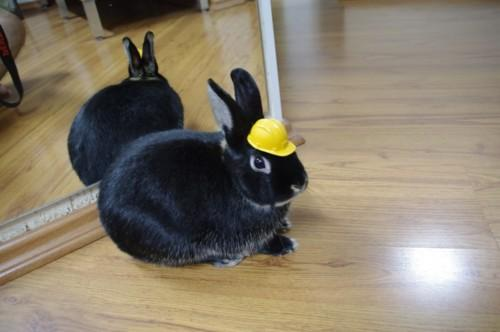
\includegraphics{{figs/bunny}.jpg}}
  }

}

%-------------------------------------------------------------------

\frame{
  \frametitle{The data}

  \parbox{\textwidth}{
    \resizebox{\linewidth}{!}{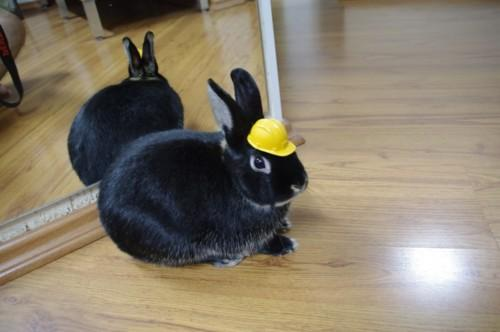
\includegraphics{{figs/bunny}.jpg}}
  }
  
}

%------------------------------------------------------------------


\frame{
  \frametitle{TF-IDF}

  \parbox{\textwidth}{
    \resizebox{\linewidth}{!}{
\includegraphics{{figs/cat}.jpg}}
  }
  
}

%-------------------------------------------------------------------

\frame{
  \frametitle{W2V}

  \parbox{\textwidth}{
    \resizebox{\linewidth}{!}{
\includegraphics{{figs/dog}.jpg}}
  }
  
}

%-------------------------------------------------------------------

\frame{
  \frametitle{LDA}

  \parbox{\textwidth}{
    \resizebox{\linewidth}{!}{
\includegraphics{{figs/cat}.jpg}}
  }
  
}

%-------------------------------------------------------------------

\frame{
  \frametitle{Another Layer}

  Train each of these on 70\%
  
  \parbox{0.34\textwidth}{
    \begin{itemize}
    \item TF-IDF
    \item W2V
    \item LDA
    \end{itemize}
  }

  Then train weights for combining probabilities on 10\%
  
}

%-------------------------------------------------------------------

\frame{
  \frametitle{Compare Scores}

  \parbox{0.34\textwidth}{
    \begin{itemize}
    \item TF-IDF \hfill 1.x
    \item W2V \hfill 1.x
    \item LDA \hfill 1.x
    \item combined \hfill 1.x
    \end{itemize}
  }
  
}

%-------------------------------------------------------------------


\end{document}
